\chapter{Grundlagen der Ökologischen Nachhaltigkeit - Henk}
Zuallererst bedarf es einer Definitition der ökologischen Nachhaltigkeit und weshalb diese überhaupt erstrebenswert ist. Die Wirtschaftsweise der Menschheit ist stehts im Wandel und unterscheidet sich von Land zu Land. Die immer gravierender werdenden Auswirkungen des menschengemachten Klimawandels haben dazu geführt, dass in den Köpfen der meisten Einwohner der Industrieländer Gier und die ``Geiz ist geil'' Mentalität lange nicht mehr attraktiv sind. Auch vor dem Hintergrund von Finanz- und Weltwirtschaftskrisen scheint die Motivation für einen grundlegenden wirtschaftlichen Wandel sogar größer denn je. Sei es Elektromobilität, vegetarische oder vegane Ernährung, Fair-Trade-Produkte, Kooperation mit Hilfsorganisationen oder Energiewende, alles soll heutzutage 'nachhaltig' sein, doch was genau ist überhaupt mit Nachhaltigkeit gemeint? \newline Der Begriff Nachhaltigkeit geht in seiner Verwendung auf den Freiberger Oberberghauptmann Carl von Carlowitz (1645-1714) und die Waldwirtschaft zurück\cite{doi:nachhaltig}. Der Kern der Aussage, in der der Begriff vorkam, war, dass laut Carlowitz in einem Wald nur so viel abeholzt werden sollte, dass dieser stets über die Kraft verfüge, auf natürliche Art und Weise nachzuwachsen. Es ging also um eine schlaue Art der Waldbewirtschaftung, die es kommenden Generationen ermöglichen sollte, ebenfalls von der kontinuierlichen Nutzung des Waldes zu profitieren. Die Definition, die bis heute am meisten Anwendung sowie Anerkennung findet und um welche es in dieser Arbeit gehen soll, ist also, dass Nachhaltigkeit generell als die Fähigkeit definiert wird, die Bedürfnisse der heutigen Generation zu befriedigen, ohne die Möglichkeiten künftiger Generationen zu gefährden, deren Bedürfnisse ebenfalls zu befriedigen. \clearpage Nun bleibt zu klären, in welche Felder die Nachhaltigkeit aus wirtschaftlicher Perspektive gegliedert wird. Aus Abbildung 2.1 lässt sich entnehmen, dass die Nachhaltigkeit sowohl sozialer, ökologischer als auch ökonomischer Natur sein kann, ich werde mich aber nur auf die Ökologie fokussieren.\newline Die Grundlage unserer Existenz besteht aus natürlichen Ressourcen. Ob veganes Sojaschnitzel, Klamotten oder unser geliebtes Smartphone, für alle Produkte wurden Wasser, Böden und Rohstoffe genutzt. Ohne diese natürlichen Ressourcen wären wir heute nicht, wer wir sind. Diese Ressourcen sind jedoch begrenzt, gerade Rohstoffe wie Erdöl und Metalle werden irgendwann aufgebraucht sein und können nicht grenzenlos zu Produkten verarbeitet werden. Das gleiche gilt für Ressourcen wie Sauerstoff und Energie. Genau diese Umstände, dass Menschen und ihr Konsum eine Auswirkumg auf die Gesamtumweltsituation haben, fällt unter den Begriff der Ökologie. 
Umgangssprachlich wird das Adjektiv ``ökologisch'' als Ausdruck für eine Haltung oder ein Agieren verwendet, das schonend mit Umweltressourcen umgeht\cite[13-23]{test123}. Wie diese ökologische Nachhaltigkeit durch moderne Technologien wie einer Blockchain-Anwendung erreicht und unterstützt werden kann, soll im folgenden prognostiziert werden.

\begin{figure}[ht!]
	\centering
	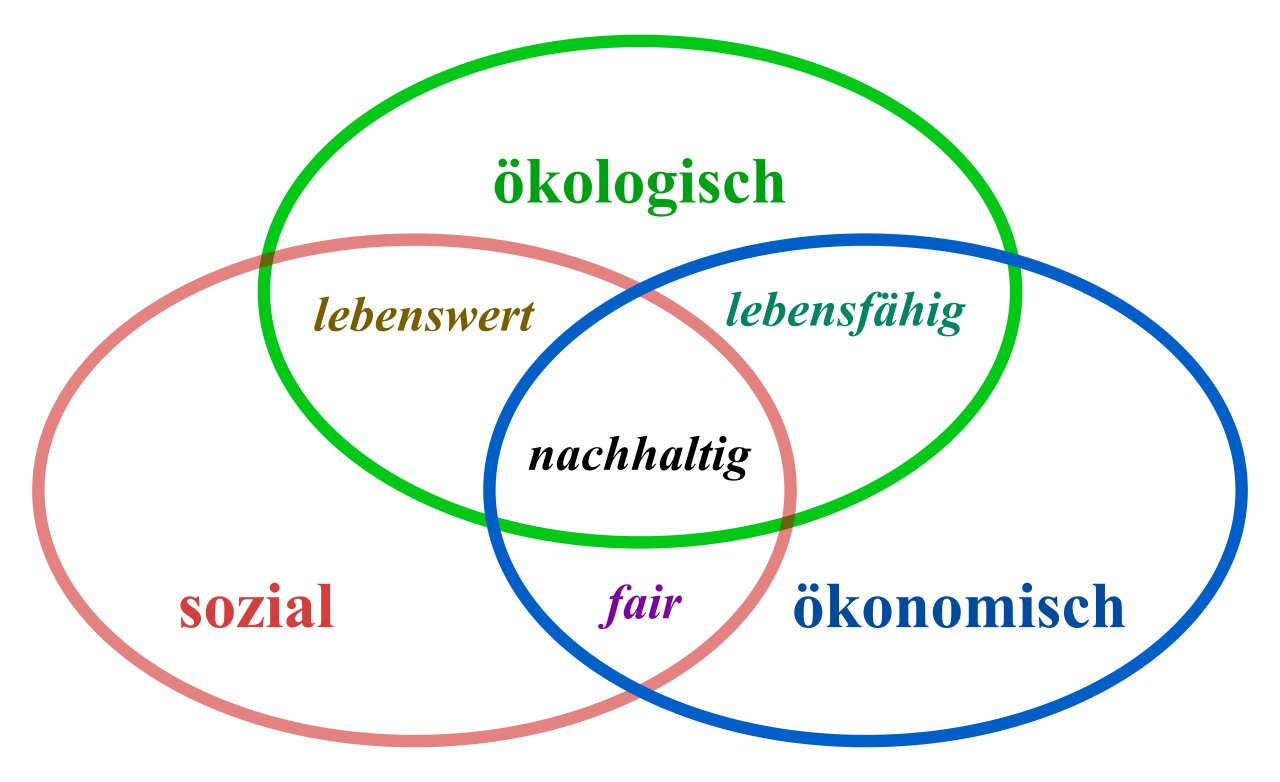
\includegraphics[width=100mm]{nachhaltig.jpg}
	\caption{Die drei Aspekte der Nachhaltigkeit\cite{oekologischeN} \label{overflow}}
\end{figure} 
\chapter{Technologische Grundlagen der Blockchain-Technologie}
\section{Mehr als nur Bitcoin - Nagi}
Wenn man sich die Statistik anschaut oder die Leute direkt fragt, ist eher Bitcoin oder Blockchain bekannt. Die Antwort dafür ist klar(https://trends.google.com/trends/explore?q=Bitcoin,Blockchain): Mit der Währung Bitcoin kann man etwas anfangen. Und ohne die Blockchain-Technologie gäbe es kein Bitcoin. Und die meisten Leute, die eine Vorstellung davon haben, was Blockchain ist, finden es schwierig zu erklären, was es genau ist. Bitcoin ist als Kryptowährung bekannt, die einige Menschen in kurzer Zeit sehr reich gemacht hat. Daher können wir verstehen, warum Blockchain weniger bekannt ist als Bitcoin.
\newline
Die Leute mögen es lieber, wenn sie über Dinge sprechen, die sie verstehen. So etwas wie Blockhain, das unantastbar oder gekauft ist, ist kein wirklich gutes Thema für die Presse oder als Thema in unseren täglichen Gesprächen. Im Gegensatz dazu kann Bitcoin, das ebenfalls unantastbar ist, zumindest online gekauft werden. Und die Presse würde wirklich schöne Titel dazu finden. Wie zum Beispiel: Dieser 18-jährige Teenager hat dank Bitcoin in 5 Jahren Milliarden von Dollar verdient (https://fee.org/articles/meet-the-teenage-dropout-who-became-a-bitcoin-millionaire/), oder der Typ, der nach diesem einen Computer sucht, auf dem er vor 10 Jahren einige Bitcoins geschürft (mined) hat und ihn sehr reich machen würde, wenn er den Computer findet .
\newline
All diese Art von Nachrichten tragen dazu bei, Bitcoin immer bekannter zu machen. Aber die Technologie hinter diesem Meisterwerk wird immer vergessen: Das gleiche Konzept, das Bitcoin im Finanzbereich sehr erfolgreich gemacht hat, könnte in vielen anderen Bereichen eingesetzt werden und mehr Wert schaffen. Beispielsweise könnten die Energieauthentifizierung und die Stromversorgung (über die wir später in einem anderen Kapitel sprechen) viel transparenter und Strom dadurch billiger werden. Aber es braucht viel Zeit, um es zu erklären. Ich meine, es ist nicht so einfach, jemanden davon zu überzeugen, etwas Geld in Bitcoin zu investieren und in ein paar Tagen reich zu sein.
\newline
Die folgenden Absätze geben eine klare Vorstellung davon, was Blockchain eigentlich ist. Es soll zunächst einen guten Überblick über einige Fachbegriffe geben und dann versuchen, Blockchain ganz einfach zu erklären. Wir werden schließlich auf die einzelnen Unterpunkte einer Blockchain eingehen. Und wir beginnen mit zwei Begriffen: Zentralisierung und Dezentralisierung, und was ist der Unterschied zwischen ihnen. 
\section{Zentral vs Dezentral - Henk}
Um das benötigte Verständnis zu schaffen, werden wir einige Grundlagen über Blockchain und Kryptowährungen klären und kurz erläutern, in welchem Zustand sich aktuelle Internetanwendungen befinden und wie diese in Zukunft aussehen könnten. \newline
Die ersten Computernetzwerke entstanden in den 1960er Jahren. Über die folgenden drei Jahrzehnte entwickelte sich das Netzwerk, welches unter dem Namen ARPANET vom Verteidigungsministerium der Vereinigten Staaten begründet wurde, zum Internet, das wir heute kennen und täglich verwenden\cite{arpanet}. Weitere 30 Jahre nachdem das Internet massentauglich wurde, bilden zentrale Datenarchitekturen immernoch die Grundpfeiler des gesamten Netzwerks. Das heißt, unsere Daten werden zentralisiert auf wenige Computer, welche als Server im Netzwerk Kopien jener Daten speichern und bereitstellen, damit sie von für uns Nutzer oder Clients stehts abrufbereit sind. Diese Praktik sollte Misstrauen hervorrufen, denn wenige, mächtige Institutionen sind somit in der Lage, wenn sie es denn wöllten, sehr effizient Daten zu manipulieren, zu löschen oder aber nur bestimmten Nutzern den Zugriff zu erlauben. Dafür müssten sie in den meisten Fällen nur genau einen Punkt im Netzwerk kontrollieren. Betrachtet man die ganze Welt, wird man schnell fündig, wie manche Regierungen von besagter Macht kurzerhand Gebrauch machen. 2017 hat die spanische Regierung genau diese Problematik ausgenutzt, um die Unabhängigkeit der Katalanen zu verhindern \cite{catalonia}.
\begin{figure}[ht!]
	\centering
	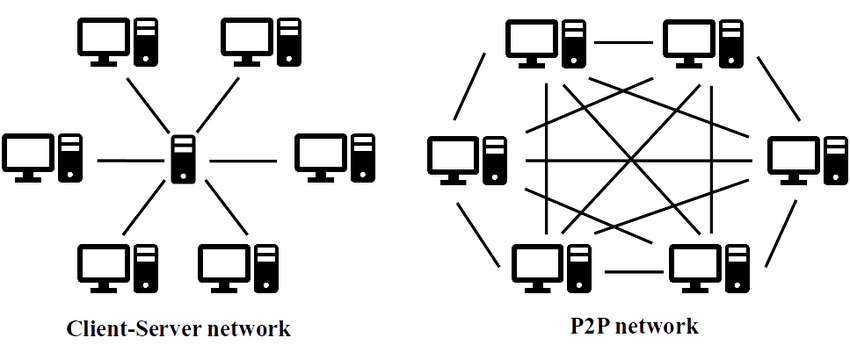
\includegraphics[width=100mm]{peer2peer.jpg}
	\caption{Vgl. Zentral vs. Dezentral\cite{p2p} \label{overflow}}
\end{figure}\newline Eine alternative Architektur ist die der Dezentralität. Diese dezentralen Anwendungen basieren auf sogenannten Peer-to-Peer-Netzwerken, in denen die Benutzer untereinander direkt kommunizieren und dies eben nicht über einen sich in der Mitte befindenden Server tun. Anwendungen dieser Art gibt es nicht erst seit 2009, dem Jahr in dem der Bitcoin vorgestellt wurde, aber mit ihm wurde ein neues Prinzip erfunden, das es anonymen Teilnehmern eines riesigen globalen Netzwerks ermöglicht, ein gegenseitiges Vertrauen zu schaffen, welches zuvor nur durch juristisch bindende Verträge oder zentrale Institutionen, also Banken oder Plattformen wie Google und Facebook, geschaffen werden konnte. Die Grundlage des Bitcoin-Protokolls ist, dass alle aktiven Teilnehmer, auch Nodes genannt, lokal eine Kopie des gemeinsamen Kursbuches (zu Deutsch ledger) abspeichern, wie es sonst nur von Banken geführt wird. In diesem Kursbuch stehen alle bisher getätigten Transaktionen seit Beginn des Bitcoins. Der Unterschied ist, dass in diesem Fall nicht ein zentraler Akteur eine einzige Kopie des Ledgers besitzt, sondern gleich alle Akteure weltweit Kopien mitführen. Es handelt sich also um ein verteiltes Kursbuch bzw im Englischen einen ``distributed ledger''. Das Bitcoin-Netzwerk wird auf den Händen dieser besagten Nodes getragen. Wollen diese Nodes aktiv neue Transaktionen ins Kursbuch hineinschreiben, so müssen sie im Bitcoin-Protokoll einen Beweis darüber vorzeigen, dass sie eine gewisse Rechenleistung erbracht haben, den sogenanngen Proof of Work. Hierdurch entsteht die Sicherheit des gesamten Netzwerks und auch dessen enorme Energielast, über welche in den Medien berichtet wird. Die verarbeiteten Transaktionen werden anschließend in Blöcke zusammengefasst und als Paket in das Kursbuch eingefügt. Es handelt sich also um eine immer länger werdende Kette aus Blöcken, daher der Begriff Blockchain. Für jeden Block, den ein Miner, also jemand der eine Node betreibt um neue Blöcke zu erstellen, an die Kette anfügt, wird er wiederum mit Bitcoins belohnt, damit ein Anreiz gegeben ist, eine horrende Stromrechnung in Kauf zu nehmen, um die Sicherheit des Bitcoin-Netzwerks zu unterstützen\cite{bitcoinWiki}.\clearpage Genau hier liegt auch aktuell der ökologisch problematische Teil des ganzen Systems. Riesige Farmen, bestückt mit tausenden sogenannten ``Mining Rigs'', also hoch spezialisierten Computer-Chips, mit welchen man sehr effizient Bitcoin minen kann, bilden die Grundlage des Bitcoins. Größtenteils befinden sich diese natürlich in Ländern in dem der Strom sehr billig ist, zum Beispiel China, was bedeutet, dass ein großer Teil der Energie, welche benötigt wird um das Bitcoin-Netzwerk zu betreiben aus Kohlekraftwerken stammt, welche natürlich einen sehr miserablen Kohlenstoffdioxid Fußabdruck besitzen\cite{miningChina}\cite{bitcoin}\cite{tokenEco}.
\section{Smart Contracts - Henk }
Die zuvor beschriebenen Programme welche vom dezentralen Aspekt der Blockchain-Technologie profitieren, basieren auf sogenannten Smart-Contracts. Das sind sehr kompakte Programme, welche wie eine normale Transaktion auch, in der jemand einen Coin von A nach B sendet, auf allen Nodes des verteilten Netzwerks gespeichert werden. Alle Mitglieder und vor allem die Miner im Netzwerk überprüfen dann, ob die jeweilige Ausführung des Quellcodes, welcher den Smart-Contract bildet, stimmt. Dieser Vorgang läuft genauso ab wie bei einer Coin Transaktion, in der überprüft wird ob der Sendende überhaupt über genug Guthaben für die geplante Transaktion verfügt, nur das in diesem Fall die zu überprüfenden Variablen aus komplexerer Logik bestehen können
\section{Konsensalgorithmus - Nagi}
\chapter{Chancen und Risiken}
\section{Risiko 1 - Samuel}
\section{Risiko - Entstehung von Elektromüll - Niels}
Wenn man sich sich mit der ökologischen Nachhaltigkeit von Blockchain auseinandersetzt, findet man viele Berichte über dessen Energieverbrauch. Dieser wurde im vorherigem Kapitel bereits behandelt und soll hier nur kurz angeschnitten werden. Im Anwendungsfall der Kryptowährung Bitcoin, wird laut einer aktuellen schätzenden Statistik \cite{de_vries_bitcoin_nodate} jährlich 121,51 Terawattstunden an Energie verbraucht damit die Geräte des Netzwerkes ihre Berechnungen des SHA-256 Hashes durchführen können. Die Hardware, welche für diesen Prozess des Schürfen (engl. Mining) verwendet wird, hat seit dem Beginn von Bitcoin vier Phasen \cite{taylor_evolution_2017} durchlaufen.
\newline
Zu Beginn wurde für das Schürfen die CPU verwendet. Ein optimiertes Modell wie das „Intel Core i7-990x“ konnte bis 33 Megahashes die Sekunde berechnen. Diese Hardware ist allerdings für den allgemeinen Gebrauch gedacht und besitzt deshalb auch eine breites Spektrum an Optimierungen für nicht, in diesem Szenario, benötigte Operationen. Durch die Leistungseinbußen aufgrund der anderweitigen Optimierungen wurde der Fokus im Jahr 2010 auf GPU’s gelegt. Da Grafikkarten bereits eine bessere Optimierung für die notwendigen mathematischen Berechnungen hatten, ließen sich mit ihnen bis zu 675 Megahashes die Sekunde berechnen. Somit haben sie bis zu 20 mal mehr Arbeit verrichten können.
\newline
Der Nachfolger der Grafikkarte kam bereits ein Jahr später und dabei handelte es sich um FPGA’s. Die Bezeichnung FPGA steht für „Field Programmable Gate Array“ und bezeichnet dabei ein Gerät mit dem sich digital benutzerdefinierte Schaltkreise darstellen lassen, welche einen viel höheren Grad der Optimierung zuließen. Dies Äußerte sich nicht in der Menge der Hashwerte, welche sie pro Sekunde berechnen konnten, sondern auch durch ihre Energieeffizienz. Ihr Nachfolger und die aktuelle bevorzugte Geräte Art sind ASIC’s, dabei steht die Abkürzung für „Application Specific Integrated Circuit”. Sie bieten nochmals einen höheren Grad der Optimierung als FPGA’s an. Besitzen allerdings den Nachteil das die Schaltkreise sich nach dem Fertigungsprozess nicht mehr anderweitig programmieren lassen. Eines der ersten Geräte konnte bis zu 60 Gigahashes die Sekunde berechnen und war damit bereits 100 mal schneller als seine Grafikkarten oder FPGA Konkurrenten. Ab diesen Zeitpunkt  war es ein Wettkampf der ASIC-Hersteller, wer die Energieeffizientesten Geräte anbieten konnte. Zur Zeit ist das Leistungsstärkste und Energieeffizienteste Gerät der „Antminer S19 Pro“ \cite{michel_rauchs_cbeci_nodate} von Bitmain mit 110 Terahashes die Sekunde.
\newline
Wie bei dem Stromverbrauch aus Kapitel 3.1 lässt sich nicht genau festlegen wie viele Geräte aktive am Bitcoin Netzwerk arbeiten. Es ist aber möglich eine Schätzung anhand der aktuellen Hashwert Rate \cite{blockchaincom_statistic_nodate} des Netzwerkes zu geben. Laut dem Stand vom 31 Mai 2021 wurden pro Sekunde 150,292 Millionen Terahashes Berechnet. Wenn nun angenommen wird das im gesamten Netzwerk nur eine Art von Gerät verwendet wird, wie Beispielsweise der „Antminer S19 Pro“, lässt das den Schluss zu das ungefähr 1,366 Millionen Geräte benötigt werden um diese Rechenleistung zu erreichen. Der „Antminer S19 Pro“ wiegt nun 13,2kg was in der Masse ein Gewicht von 18,0312 Kilotonnen ergibt. Wie Alex de Vires \cite{de_vries_renewable_2019} bereits in der Zeitschrift Joule vom April 2019 erwähnt hat ist das Schürf-Equiqment auch von „Koomeys Gesetz“ betroffen, welches besagt das sich die Leistungsfähigkeit alle 18 Monate verdoppelt. Da die Teilnehmer des Netzwerkes nun untereinander im Wettstreit stehen um am schnellsten den Hash-Wert des nächsten Blocks zu berechnen und damit den Bitcoin-Gewinn zu bekommen, müssen diese kompetitiv bleiben, was sich äußert indem veralteten Geräte durch performantere Modelle ersetzt werden. Hier wird die Herstellung von ASIC Geräten zum Problem, da diese nicht anderweitig verwendet werden können, werden sie zu Elektromüll. In dem Jahr 2019 wurden 17,4% \cite{forti_global_nodate} des weltweiten Elektromüll offiziell recycelt. Dadurch ist zu erwarten das aus den 18 Kilotonnen nur 3,132 Kilotonnen offiziell wiederverwertet werden. Bei dem Rest ist zu befürchten das er auf Mülldeponien gelagert, in Seen und Flüssen gekippt oder schlichtweg verbrannt wird.
\newline
Es besitzt aber nicht nur der Bitcoin das Potenzial viel Elektromüll zu erzeugen. Am 19 März 2021 ist eine neue Kryptowährung namens Chia offiziell in den Betrieb genommen worden. Diese Währung hat als Konsens-Algorithmus nicht „Proof of Work“ sondern „Proof of Space“.  Bei „Proof of Space“ wird anstatt Rechenleistung, Speicherplatz verwendet. Es wird  ein sogenannter Plot erstellt, der schließlich einen gewissen Bereich an Speichert in Anspruch nimmt. Ein Plot besteht aus Zahlen, welche anhand von kryptografischen Berechnungen erstellt wurden. Dieser Prozess wird bei Chia als „Plotting“ bezeichnet. So ein Plot kann eine endgültige Größe von 108,9 GB bis zu 949,3 GB \cite{hoffman_plot_2021} besitzen. Dabei handelt es sich um die finalen Werte die nach dem komprimieren der Daten benötigt werden. Während des Vorganges wird temporär das 2,5 fache an Speicher benötigt. Ein Plot würde Beispielsweise während des Vorganges auf 256,6 GB anwachsen und nach dem Komprimieren nur noch 108.9 GB benötigen. Der gesamte Vorgang des Plotting benötigt durchschnittlich 9 bis 12 Stunden \cite{hoffman_chia_2021}. Von dem Netzwerk wird alle 20 Sekunden eine Zahl verlost und der Teilnehmer, welcher diese Zahl in seinem Plot findet ist berechtigt den Nächsten Block der Kette zu verifizieren und damit den Gewinn zu bekommen. Das Warten auf eine passende nennt sich „Farming“ in Chia und ist in Kombination mit Plotting das äquivalent zum Schürfen in Bitcoin.
\newline

Hier kommt Tabelle!!! (TODO)

In der Tabelle sind 10 gängige Modelle von mindestens 1 Terabyte großen SSD’s aufgelistet. Zu jedem dieser Modelle ist die dazugehörige Schreibleistung in Terabyte angegeben wie sie aus dem Datenblätter der Produkte zu entnehmen war. In der Spalte „Parallele Plots“ ist  die Anzahl der Vorgänge angegeben, welche gleichzeitig mit der Speichergröße des Modell und 32 GB Arbeitsspeicher durchgeführt werden können. Die letzte Spalte gibt ein ungefähres Zeitfenster an an dem die gesamte Schreibleistung des Modell erreicht ist. Ab dem Zeitpunkt kann es zu Schreibfehlern auf der Festplatte kommen, wodurch diese nicht mehr für den Gebrauch verwendet werden kann. Die Berechnung es „End of Life“ (EOL) ist mit den Vorgaben geschehen das ein Plot temporär 256,6 GB an Daten schreibt und der Vorgang Konstant 9 Stunden benötigt. Bei den Modellen hat sich eine Durchschnittliche Dauer von 26 Monaten bis zum erreichen der Schreibleistung ergeben, sie können also effektive 2 Jahre und 2 Monate verwendet werden bevor sie ausgetauscht werden müssen.
\newline
In den zwei Anwendungsfällen von Blockchain haben wir uns angesehen weshalb es zu der Entstehung von Elektromüll kommen kann. Es liegt daran das ein kompetitives Verhalten zwischen den Teilnehmern eines Netzwerkes entsteht, welches dafür sorgt das die benötigte Ressource, welche den Konsens-Algorithmus befriedigt, aufgebläht wird. Im Falle von Bitcoin ist es die Rechenleistung und bei Chia der Speicherbedarf. Da die Gewinne der Teilnehmer unabhängig von der Größe des Netzwerkes sind, sondern nur ihre Verteilung sich ändert, muss jeder Teilnehmer immer mehr Ressourcen zur Verfügung stellen damit er seine Chancen auf einen Gewinn halten kann. Dieses Verhalten kann bei jeder Blockchain Implementierung erwartet werden, wo die Teilnehmer durch einen Gewinn motiviert werden an dem Netzwerk teilzunehmen und der Konsens-Algorithmus als Flaschenhals eine spezielle Ressource vorgibt.
\section{Chance: Lieferketten Transparenz - Henk}
Als Kontrast zu den vorhergegangenen Risiken gibt es auch große Chancen die der globalen Bevölkerung ein besseres Leben verschaffen können. Eine dieser Chancen ist die ermöglichung von mehr Transparenz und Authentizität, denn
Transparenz ist ein Begriff, der immer mehr an Bedeutung gewinnt. Gerade entlang der Liefer-und Versorgungskette von Konsumgütern würde eine Erhöhung der Transparenz eine Menge von Vorteilen bringen. Der Endverbraucher hat aktuell kaum eine Chance festzustellen, ob Dinge wie Umweltverschmutzung, Betrug oder gar Menschenrechtsverletzungen entlang der Produktionskette des Produktes entstehen, welches er vor sich im Supermarktregal sieht, denn auf die Verpackung passt einfach nicht genügend Information. Nichtsdestotrotz kommt es immer wieder vor, dass solche Negativumstände, nachdem viele Menschen ein Produkt gekauft haben, ans Licht kommen. Dies macht es sowohl Privatpersonen als auch Firmen schwer, nachhaltige Konsumentscheidungen zu treffen. In den aktuell verwendeten Systemen fehlen die Mittel zur verlässlichen Überprüfung von Verhalten entlang der Lieferkette. Die zuvor beschriebenen dezentralen Anwendungen, welche über Smart-Contracts auf einer grünen Blockchain laufen könnten, erzeugen hier Hoffnung, denn mit ihnen ist es möglich, ein bisher unerreichtes Niveau an Transparenz zu schaffen. Durch die Eigenschaft der transparenten Abspeicherung und der Unveränderbarkeit der dezentral abgelegten Daten wird es für Teilnehmer, fast unmöglich nachträglich falsche Fakten zu schaffen, sofern die Informationen welche ursprünglich eingespeist worden sind denn der Wahrheit entsprechen. Lieferketten sind also ein gutes Beispiel, anhand dessen man aufzeigen kann wie Blockchain-Lösungen die Nachhaltigkeit fördern könnten. Eine Lieferkette ist ein komplexes Netzwerk, das aus seperaten und räumlich voneinander getrennten Institutionen besteht. Diese Instituitonen wiederum befinden sich im ständigen Austausch von Produkten, Zahlungen und Daten. Blockhain-Anwendungen könnten hier ansetzen, um die Herkunft von Gütern und Dienstleistungen entlang der Kette nachvollziehbarer zu machen. Der zuvor erwähnte Austausch von zentraler durch dezentrale Blockchain-Architekturen kann auch hier enorme Vorteile bringen. Beispielsweise könnten Datenredundanzen und Dateninkonsistenzen, welche durch multiple Dokumentenkopien entstehen, vermieden werden, indem nur eine Version eines Dokuments im Blockchain-Kursbuch vermerkt wird. Auf Dauer kann hierdurch eine Echtzeit-Transparenz entlang der Lieferkette erreicht werden, sofern alle Teilnehmer software auf der Blockchain basieren und unter der Voraussetzung, dass die Blockchain-Lösungen durch Big Data und das Internet der Dinge (IoT) verknüpft werden. Denn ein wichtiger Aspekt ist, dass man den Daten, welche in die dezentralen Anwendungen gespeist werden, von Beginn an vertrauen kann, und dass dadurch IoT-Lösungen unverfälschte Echtwelt-Daten liefern.\newline
Die Herkunft von Gütern und Dienstleistungen ist ein Beispiel für Information welche transparenter kommuniziert werden kann. Wenn Güter ihre Endstation erreichen, wissen die meisten Käufer und Verkäufer nichts über den wahren Ursprung der hergestellten Ware oder über deren Inhaltsstoffe bescheid. Würde man als Verbraucher zum Zeitpunkt des Kaufs mehr Informationen erhalten, so hätte man deutlich mehr Möglichkeiten, aber auch mehr Verantwortung, über die Produktonsweise und Herkunft diverser Güter mitzubestimmen. Man könnte sich ein deutlich besseres Bild darüber machen ob das Gut umweltbelastend produziert worden ist und unter welchen Bedingungen dies geschehen ist. \newline Ein weiteres Beispiel ist die Nachvollziehbarkeit des Preises, denn mangelt es an ihr sowie an der Nachvollziehbarkeit der Kosten, die durch etwaige Zwischenhändler aufgeschlagen werden, so werden Endkonsumenten erheblich daran gehindert zu verstehen, wer welche Einnahmen in einer Lieferkette verzeichnen kann, oder auch, wie die Arbeitsbedingungen für die Produzenten sind\cite{lieferkette}.\newline Auch vor Plagiaten kann diese erhöhte Transparenz schützen. Mehr gesicherte Informationen machen es schwieriger, den Kunden von der Echtheit des gefälschten Produkts zu überzeugen. Auch dies würde die ökologische Nachhaltigkeit fördern, denn meist werden Plagiate unter umweltverschmutzenden Bedingungen mit minderer Qualität der Ressourcen geschaffen.\newline Eine Blockchain, die sich nur mit der Transparenz von Lieferketten beschäftigt und Anwendungen unterstützt, die man schon heute schon ausserhalb Deutschlands im alltäglichen Gebrauch finden kann, ist VeChain. Produkte, welche durch VeChain-basierte Anwendungen transparenter gestaltet werden, verfügen über einen NFC-Chip, welcher auf der Verpackung klebt. Öffnet man die Verpackung, geht der NFC-Chip kaputt, was dem Endverbraucher garantiert, dass der Inhalt unverändert die Fabrik verlassen hat. Scannt der Kunde den Chip mit seinem Handy, so erhält er ausführliche Informationen über das Produkt, welchen er mehr vertrauen kann als einem gedruckten Werbespruch auf der Verpackung oder einem vermeintlich glaubwürdigen Klimasiegel \cite{vechain}\cite{veDoc}.
\section{Chance 2 - Nagi}

